% This template was originally by R. Jacob Vogelstein
% Updated on March 1, 2010 by Noah J. Cowan
% Updated by Brian D. Weitzner, April 29, 2014

\documentclass[12pt,oneside,final]{thesis}

\usepackage{cite}
\usepackage{amsmath}
\usepackage{amsfonts}
\usepackage{amssymb}
\usepackage[pdftex]{graphicx}
%\usepackage{pdftex} 
\usepackage{wrapfig}
\graphicspath{{./figs/}}
\DeclareGraphicsExtensions{.eps}
\usepackage{fixltx2e}
\usepackage{array}
\usepackage{times}
\usepackage{fancyhdr}    % Use nice looking headers along with the required footer page numbers   
\usepackage{longtable}
%\usepackage[hypertex]{hyperref}
\usepackage{multirow}

\usepackage{currvita}

\usepackage{fancyhdr}    % Use nice looking headers along with the required footer page numbers   
%\usepackage[hypertex]{hyperref}

%Define the header/footer style
\pagestyle{fancy}
\fancyhf{}
\setlength{\headheight}{15pt}
\lhead{\leftmark}
\cfoot{\thepage}
\renewcommand{\headrulewidth}{0pt}
\fancypagestyle{plain}{% Redefine ``plain'' style for chapter boundaries
\fancyhf{} % clear all header and footer fields
\fancyfoot[C]{\thepage} % except the center
\renewcommand{\headrulewidth}{0pt}
\renewcommand{\footrulewidth}{0pt}}

%\tolerance=10000

\long\def\/*#1*/{}

\renewcommand{\rmdefault}{iwona}

%\makeglossary % enable the glossary

\begin{document}

\title{
\begin{Large}
A TALE OF TWO VERTICES: \\
\end{Large}
Production and Decay of the HVV Vertex at the LHC
}
\author{Ian J. Anderson}
\degreemonth{}
\degreeyear{2015} 
\dissertation
\doctorphilosophy
\copyrightnotice


% add your chapters, best way is to have separate TeX files for each chapter
%% FRONTMATTER
\begin{frontmatter}

% generate title
\maketitle

\begin{abstract}
Something about the Higgs.

\vspace{1cm}

\noindent Primary Reader: Andrei Gritsan\\
Secondary Reader: Someone Else
\end{abstract}

\begin{acknowledgment}
Unsurprisingly, it's difficult for me to acknowledge all those who have been there in some form or another along my journey to this point. Not for spite or pride, but for brevity; there are neither enough words nor pages for me to adequately thank everyone in name or deed. I am eternally grateful for each of you, this is only a small slice thereof. 

First and foremost, I would like to thank my advisor, Andrei Gritsan. Over the past few years that I've known and worked with you, we've published a number of different results that have all taken countless shared hours, conversations, and emails. What I've learned from our talks -- either in physics, in communication skills, or in self-determination -- has been invaluable. Without your intuition, encouragement, and support, I wouldn't be where I am today. 

I must also thank all of my colleagues and collaborators in the JHU HEP group. I owe much of what has been achieved and who I have become in the last few years to you. Morris, Petar, Barry, and Bruce have each supplied words of advice and inspiration over my time at Hopkins. Yanyan, Nhan, Andrew, Sara, and Meng: your ample experience and boundless patience was a godsend. To Candice and Heshy, I feel so lucky to have worked alongside you. For Marc, Dave, Nick, Kevin, Yongjie, Alice, Raymond, and Yaofu: our debates, collective troubleshooting, and general companionship has been my sustenance. And to Chris and Ulascan, there is no earthly way these results would have made it to publication without our discussions, arguments, and sweat. Knowing that we were in this together made it not only feasible but endurable.

To those JHU colleagues now elsewhere, especially Kirill, Fabrizio, and Markus, I'm honored to have collaborated with you. For my fellow CMS members abroad, especially Roberto, Nicola, NDF, Michalis, and all the collaborators from the Higgs and ZZ4L group, your expertise and assistance has been crucial, both to myself and the field. To the administrative staff in Bloomberg -- Carm, Pam, Kelley, Brian -- I'm so grateful for everything you have done to keep this program afloat. 

To Chris, Matt, Sean, and David: your combined theoretical expertise is awe-inspiring and our various discussions -- on physics or far afield -- have been immeasurable and I'm honored to call you friends. Tristan, Kate, Grace: our adventures through these past few years are some of the most memorable experiences I've ever had and I will always treasure them. For Matt, Justin, Nik, Keith, Derek, JT, and Mike, thank you for all of the great -- occasionally inane, though nothing if not interesting -- conversations and good times we've had together. To KFC, thank you for all the  -- almost always inane -- phone calls, late nights, and arguments over the years.

Lastly, the support and understanding from my family has been my rock through troubled seas. Throughout my life, there have been periods of unease, stress, and heartbreak. And yet, I am always in awe at your resilience and limitless love. Truly, to my parents, to my siblings, to my aunts and uncles and cousins, I owe my life and who I am to you all.
Finally, to my wonderful girlfriend Nassira, I cannot imagine what my life would have been without you. That I could have been fortunate enough to meet you, to share this journey next to you, to grow with you - I feel so privileged and I can't wait to see what we do next. 
\end{acknowledgment}

\begin{dedication}
In so many ways, this thesis is dedicated to Sophie, Jane, Jeanie, Grammy, Louise, Marie, Ritchie, Herk, and Lorraine.
\end{dedication}

% generate table of contents
\tableofcontents

% generate list of tables
\listoftables

% generate list of figures
\listoffigures

\end{frontmatter}

\chapter{Introduction}
\label{sec:intro}
\chaptermark{Introduction}

\begin{center}
\begin{footnotesize}
{ \it{``It has long been an axiom of mine that the little things are infinitely the most important."}}\\
``The Memoirs of Sherlock Holmes", Arthur Conan Doyle\\
\end{footnotesize}
\end{center}

\section{Theoretical Motivation}
\label{sec:Introduction}

Needless to say, in some sense, a discovery seemed inevitable. Near Geneva, beneath the foot of the Jura Mountains, the Large Hadron Collider (LHC) has been accelerating protons at higher energies than any collider prior, continuing the fruitful lineage of technological advancement and scientific discovery from earlier particle accelerators. On July 4, 2012, in a joint announcement from CMS and ATLAS, the organizations of the two respective general purpose detectors at the LHC, it was announced that a Higgs-like boson\footnote{Although it is now considered ``a Higgs boson", contemporarily it was deemed ``a Higgs-like boson" until further study could be done.} was observed which opened a new window to probe the foundations of the universe. The genesis of this announcement can be traced to ancient Greece and India with the origins of atomism - the postulate that there exist fundamental, unbreakable constituents that make up all matter - through the discovery of quantum mechanics to today. The Standard Model (SM) is the current answer proffered by particle physicists for the underpinnings of matter in our universe. This discovery appears to be the observation of the last remaining piece of this model.

Conceived in the 1970s, the SM has been one of the most successful scientific models\footnote{The only possible usurper is special relativity which underlies some of the mathematics of the SM.} ever. Precision tests have repeatedly agreed with SM predictions and fundamental particles which were not yet observed at the time of conception have since been discovered. The Standard Model's particles and their interactions, along with how they act in the aggregate, can explain nearly all phenomena across any size or time frame in our universe. But, as we will see in Sec.~\ref{sec:SMpreLHC}, there still remain large unanswered questions which we may hope to probe by looking in detail at this new boson.

\subsection{Our Cast of Characters: Fundamental Particles}
\label{sec:FundParticles}

Broadly, the Standard Model consists of a series of point particles with only a few basic characteristics: spin, charge, and mass.

Spin can be thought of as the intrinsic angular momentum of a particle. It can only take integer or half-integer values, which is used to classify particles into two categories: Bosons have integer spin while Fermions have half-integer spin. This classification isn't arbitrary; the spin determines the general role of that particle. Fermions obey Fermi-Dirac statistics and therefore cannot occupy identical energy states. These are the building blocks of all the observed material in the universe. Bosons instead obey Bose-Einstein statistics -- they are permitted to occupy identical energy states -- and make up the force carriers. If fermions are the pieces, bosons are the glue that binds them.

The particles can interact through any of the four observed forces: Electromagnetism, the Weak and Strong forces, and Gravity. Gravity is a bit problematic and not integrated into the Standard Model (see Sec.~\ref{sec:SMpreLHC}), but the other three forces are. We can further differentiate the fermions based on what forces they interact with. Fermions that interact with the strong force are called quarks, whereas leptons do not. How strongly these fermions interact with a given force is quantified in the concept of charge. Traditionally, when we use the term "charged" in reference to a particle, it refers to whether it interacts with electromagnetism. There are three charged leptons: the electron has unit negative charge as do its two heavier cousins, the mu and the tau. There are also three uncharged leptons called neutrinos: the electron neutrino, the mu neutrino, and the tau neutrino. All quarks are charged; the up, charm, and top quarks (up-type) have charge of +2/3 while the down, strange, and bottom quarks (down-type) have charge -1/3. The force carrier of electromagnetism is a massless, uncharged boson called the photon. These properties allow photons to travel infinitely, such that particles can interact electromagnetically over very long distances.

The weak and strong forces interact at much smaller distances, like inside nuclei of different atoms. For the strong force, the analogy of electromagnetic charge isn't simply positive or negative. Instead, particles can have color charge, which can be red, blue, or green. Quarks are the only colored fermions and the gluon is the strong force carrier. Gluons are massless, but contrary to the photon, gluons are colored so they will interact with other gluons. As a result, the strong force exhibits a property called confinement, where colored combinations of particles are unstable so quarks or gluons cannot be directly observed (see Sec.~\ref{sec:hadronization}) and thus the strong force doesn't interact over long distances. Instead, quarks tend to come in groups of two (mesons) or three (baryons)\footnote{There are some experimental results involving tetra- and pentaquarks, but they are very rare and fall well outside of the scope of this thesis.}.

If we look at these fermions, we see groups of three: three charged leptons, three uncharged leptons, three up-type and three down-type quarks. Can a fermion change from one group to another? What about to another fermion in the same group? Through the weak force, quarks can change from up-type to down-type (and vice-versa), i.e. the charm quark can decay into the down quark or the strange quark. Further, charged leptons can move from one to another, so the muon can decay into the electron. The force carrier for this decay is the W boson, which can be either positive or negatively charged. Also associated with the weak force is the Z boson, which is not charged but can still transfer momentum. But if the strong force is distance limited by confinement, why does the weak force only act over short distances? If we look at the mathematics of the weak force, it is identical to electromagnetism. So why doesn't it act like electromagnetism?

Finally, we come to mass. The reason that the charged leptons or up-type quarks aren't fully interchangeable is because they vary drastically in their mass. This has demonstrable impact on how a particle will act, as particles with higher mass will decay to those allowed which have lower mass. A muon is roughly 200 times more massive than the electron, so a muon will quickly decay to an electron. Similarly, the mass of the top quark is much heavier than any other quark, so it has a very, very short lifetime. The weak force therefore acts differently than electromagnetism because the photon is massless while the W and Z bosons are massive; the W and Z will quickly decay, usually to a pair of fermions. As a result, the first generation of fermions -- those with lowest mass: the electron, the electron neutrino, the up quark, and the down quark -- are the most stable. With just these three particles, we can make basic protons (two ups and a down) and neutrons (two downs and an up) which can be combined with the electron to form all of the atoms in the periodic table.

There is one more complication in the Standard Model. All of the particles listed so far make up matter. In addition, there are antiparticles which have the same mass, but the opposite properties. The anti-electron is called the positron as it is positive. Anti-quarks have the same name but with a bar on top, so $\bar{u}$ is the anti-$u$. Further, anti-quarks can have color of anti-red, anti-green, and anti-blue. Mesons, for example, are a quark and anti-quark pair which add up to a colorless state. As the name implies, when antimatter and matter come in contact with each other, they annihilate, converting into force carriers which can then transform into other particles. As a corollary, force carriers can split into matter and antimatter. So a proton is not just two up quarks and a down quark, but it also the interacting gluons and a sea of temporary quark-antiquark pairs, popping in and out of existence.

But why do the W and Z bosons have mass? For that matter, if the top and up have otherwise identical properties, why is the top's mass over 75,000 times greater than the up? If matter and antimatter annihilate when they collide, why must there have been more matter than antimatter? And what about gravity? These are the deeper questions of the Standard Model. Fortunately, there are possible answers that, if correct, would leave signatures we could find in particle accelerators.

\subsection{The Story: The Status of the Standard Model Before the LHC}
\label{sec:SMpreLHC}

From a mathematical perspective, the Standard Model is built off of symmetries. 

\section{Summary}
\label{sec:intro_summary}
\chapter{Experimental Setup}
\label{sec:expt}
\chaptermark{Experimental Setup}

\begin{center}
\begin{footnotesize}
{\it{``I'm going to find it and I'm going to destroy it. I don't know how yet, maybe dynamite."}}\\
Steve Zissou, ``The Life Aquatic with Steve Zissou"
\end{footnotesize}
\end{center}

\section{The Large Hadron Collider}
\label{sec:LHC}

In Sec.~\ref{sec:introduction}, we saw that although the Standard Model was tested robustly before the LHC turned on, the Higgs boson had not yet been discovered and there are still unanswered questions not covered under the Standard Model that should lead to new physics. For many decades, the primary tool of discovery in experimental particle physics is the particle accelerator. In rudimentary terms, two particles are accelerated towards each other and the byproducts of their collisions are studied to look for new particles. There are two categories of particle accelerators, leptonic and hadronic: leptonic colliders have electron-positron collisions while hadronic colliders use proton-proton or proton-antiproton collisions. As discussed, protons are made up of a sea of different particles at different energies which makes it difficult to know the exact initial conditions of a collision. A leptonic collider, on the other hand, can tune the initial energy of the collisions quite well to a particular value. However, as argued in Sec.~\ref{sec:findinghiggs} and \ref{sec:findingBSM}, the energies of the unobserved particles were unknown so any search must be done over a wide range which encourages the use of hadronic collisions. Further, the range should extend beyond that of the previous highest energy hadronic detector, the Tevatron at Fermilab which had a maximum center-of-mass energy up to about 2 TeV (2000 GeV).

The Large Hadron Collider was designed with these characteristics in mind: a 27-kilometer circular accelerator for proton-proton\footnote{Heavy ions can also be accelerated in the LHC, leading to interesting research for the strong force, but this is outside the scope of this thesis.} collisions that can reach up to energies of 14 TeV. Bunches of protons are injected at 450 GeV from the Super Proton Synchrotron, an earlier proton-proton accelerator that found direct evidence for the $Z$ boson~\cite{}. Once reaching the LHC, a series of 1232 superconducting dipole magnets with radio frequency cavities increase the energy of the protons as they move around the ring. As the bunches accelerate, the protons will tend to diffuse, which is corrected by thousands of additional magnets (quadrupole, octopole, etc). Each bunch of protons in the LHC contains $1.15\times10^{11}$ protons and each run contains 2808 bunches. These seemingly high numbers are required to probe the highest energies and rarest interactions expected at the LHC.

To quantify how rare an event is, physics utilizes the concept of \textit{cross-section} ($\sigma$). This is best illustrated by comparing the protons to a flow of ball bearings: as they pass by one another, the likelihood that any proton strikes another is proportional to the size of the ball bearings. Similarly, in quantum physics, the likelihood of an event is determined by its cross-section, typically written in units of \textit{barns} (b) where $1$ $\mathrm{b}$ $=$ $10^{-28}$ $\mathrm{m}^2$. The interesting processes to be probed at the LHC have cross-sections ranging from the order of picobarns ($1$ $\mathrm{pb}$ $=$ $10^{-12}$ $\mathrm{b}$) to fractions of femtobarns ($1$ $\mathrm{fb}$ $=$ $10^{-15}$ $\mathrm{b}$).

Particle accelerators use \textit{luminosity} ($\mathcal{L}$) to indicate how many events of a given cross-section should be expected per second, such that $\frac{dN}{dt}=\mathcal{L}\sigma$. The luminosity can be defined in terms of the accelerator's parameters:
\begin{equation*}
\mathcal{L} = \frac{\gamma f k_{B}N_p^2}{4\pi \epsilon_{n} \beta^{*}}F
\end{equation*}
where $\gamma$ is the Lorentz factor corresponding to how fast the particles are moving, $f$ is the frequency that the protons revolve through the LHC, $k_{B}$ is the number of bunches, $N_p$ is the number of protons in a bunch, $\epsilon_n$ (normalized transverse emittance) and $\beta^{*}$ (betatron function at the point of interaction) both relate to the physical size of the beam, and $F$ is the reduction factor caused by the crossing angle of the beams. Relevant design parameters are also found in Table~\ref{tbl:LHCLumi}. Ultimately, the design luminosity of the LHC is $\mathcal{L} = 10^{34}$ $\mathrm{cm}^{-2}\mathrm{s}^{-1}$ which corresponds to about 1 billion proton-proton interactions per second. Typically, the amount of data collected by a particle detector is written as the time-integrated luminosity, in units of $fb^{-1}$, to gauge how many events of a given cross-section should be expected. For example, in 10 $\mathrm{fb}^{-1}$ of data, one would expect 10 events for a cross-section of 1 $\mathrm{fb}$.

\begin{table}[htp]
\begin{center}
\begin{tabular}{|c|c|c|}
\hline
Number of bunches & $k_B$ & 2808 \\
\hline
Number of protons/bunch & $N_p$ & $1.15\times10^{11}$ \\
\hline
Bunch separation & & 25 ns \\
\hline
%Betatron Function at IP & $\beta^{*}$ & 0.55 m \\
%\hline
%Normalized Transverse Emittance & $\epsilon_n$ & 3.75 $\mu\mathrm{m}$ \\
%\hline 
Design Luminosity & $\mathcal{L}$ & $10^{34}$ $\mathrm{cm}^{-2}\mathrm{s}^{-1}$ \\
\hline
\end{tabular}
\caption{Design Parameters of the LHC}
\end{center}
\label{tbl:LHCLumi}
\end{table}%

After reaching the desired energy, the proton bunches are permitted to interact at four crossing points. Each of these points is the cite of a detector on the LHC: CMS (The \textbf{C}ompact \textbf{M}uon \textbf{S}olenoid), ATLAS (\textbf{A} \textbf{T}oroidal \textbf{L}HC \textbf{A}pparatu\textbf{s}), ALICE (\textbf{A} \textbf{L}arge \textbf{I}on \textbf{C}ollider \textbf{E}xperiment), and LHCb (\textbf{LHC} \textbf{b}eauty Experiment). CMS and ATLAS are general detectors for proton-proton interactions, while ALICE and LHCb use the protons to collide with heavy-ion targets to look deeper into the intricacies of the strong force. The remainder of this chapter will detail CMS and how it looks for particles like the Higgs.

\section{Our Setting: The Compact Muon Solenoid}
\label{sec:CMS}

The Higgs Boson and theorized particles in BSM physics are expected to be unstable and rapidly decay to the particles of the Standard Model, so it's unsurprising that the design requirements of the CMS are built around accurately detecting these particles and characterizing their energies and momenta. To collect the most information about these events, the detector should be designed to record all relevant decays so that the full kinematics could be reconstructed. This is the idea behind a \textit{hermetic} detector, where different sub-detectors are nested to capture information about any particle observed and characterized by what sub-detectors they interact with. A detailed view of the CMS detector is seen in Figure~\ref{fig:ExplodedCMS}. This section will overview the subsystems, where further details are found in the CMS Technical Design Reports~\cite{,}.

\begin{figure}[htbp]
\begin{center}
\includegraphics[width=.9\linewidth]{Experiment/figures/ExplodedCMS.pdf}
\caption[The CMS Detector with Sub-Detector Systems]{The CMS detector is built around a superconducting solenoid, with the muon system on the outer shell while the tracker and calorimeter systems are inside the solenoid.}
\label{fig:ExplodedCMS}
\end{center}
\end{figure}

\subsection{Coordinates and Conventions for the CMS}
\label{sec:CoordinateConventions}

To unambiguously define locations for components or events in the detector, a standard coordinate system is used such that the origin is centered at the nominal collision point. In cartesian coordinates, the $y$-axis is defined to be vertically upward while the $x$-axis is points toward the center of the LHC. However, given that the detector is cylindrically symmetric, directions are commonly defined using $\phi$ and $\eta$. $\phi$ is the azimuthal angle starting from the $x$-axis in the $x-y$ plane. $\eta$ is the \textit{pseudorapidity} where $\eta=-\ln\tan(\theta/2)$, $\theta$ being the polar angle measured from the $z$-axis. Momentum and energy are then broken into their transverse ($p_T,E_T$) and longitudinal ($p_z,E_z$) components. Given that the beam is along the axis which would cause a large background, the particles that have large $p_T$ or $E_T$ (or in the case of searching for energy imbalance, $E_T^{miss}$) should be the easiest to identify.

\subsection{Subsystems in CMS}
\label{sec:CMSSubsystem}

\subsubsection{The Magnet}
\label{sec:Magnet}

One way to categorize the decay products is to look at their charges. Any charged particle will have a curved trajectory in a magnetic field, where the direction is related to the sign of the charge and the scale is proportional to the momentum. Given the large energies and desired precision of the momenta, the field strength must be very strong and consistent. CMS uses a 12.9m long, 5.9m in diameter superconducting solenoid with a designed field strength of 4T, or about 100,000 times that of the Earth. An iron return yoke is used in larger to guide and return the field. In doing so, the direction of the magnetic field will be antiparallel and of lower magnitude in the muon systems compared to the field in the calorimeters and tracking systems.

\subsubsection{Muon System}
\label{sec:MuonSystem}

Muons are one of the cleanest signatures to identify and thus crucial for finding new physics. Electrons are common byproducts of many decays and can be stopped in dense material. Taus are much rarer, but have a very short lifetime and thus decay in the inner detector. Quarks cannot be observed individually. Neutrinos aren't charged and very difficult to detect as they only interact via the weak force. Muons, on the other hand, are charged, heavy leptons that have long enough lifetimes to pass through the outer reaches of the detector. Because of these properties\footnote{For exactly the same reason, this is why the LHC is deep underground. Cosmic rays commonly hit the Earth's atmosphere and shower particles observed to the surface. Although nearly all particles can be shielded without much material or decay in the upper atmosphere, muons will commonly penetrate the surface and need hundreds of meters of depth to lessen this background.}, muons that come from collisions are measured from three different sub-systems to accurately measure their kinematics. 

\begin{figure}[htbp]
\begin{center}
\includegraphics[width=.7\linewidth]{Experiment/figures/MuonSystem.pdf}
\caption[Arrangement of Detectors in CMS Muon System]{Vertical slice of CMS showing one quarter of the muon system. The three different devices used are labeled: Drift Tube (DT) chambers, Cathode Strip Chambers (CSC), and Resistive Plate Chambers (RPC).}
\label{fig:MuonSystem}
\end{center}
\end{figure}

On the outer edge of the detector, three types of detectors are used to measure muons. The layout of the different types of detectors can be seen in Fig.~\ref{fig:MuonSystem}. Away from the beam ($|\eta|<1.2$), along the barrel, four layers of 250 drift tube (DT) chambers are used. Each chamber is composed of a positively charged wire in a volume filled with gas. As the muon moves through the chamber, the gas becomes ionized and the electrons drift toward the wire. The position of the muon can then be tracked by where the electrons were observed to drift. Closer to the beam line (up to $|\eta|<2.4$), in the endcaps, four layers of 468 trapezoidal shaped cathode strip chambers (CSC) are placed. Each CSC is made of seven layers of metal, inlaid with a plane of cathode strips and anode wires nearly perpendicular to the strips. The gaps are filled with a gas that will ionize when any charged particle passes through, causing an electron avalanche which will charge anode wires and cathode strips near the trajectory, allowing spatial reconstruction at each layer.

Finally, in both the barrel and endcap ($|\eta|<1.6$), 1080 resistive plate chambers (RPC) are used to in conjunction with the DTs or CSCs. Each RPC consists of two very narrow chambers (2mm thick x 130cm long) filled with gas with anode and cathode plates made of bakelite, which has a very high resistivity. As with DTs or CSCs, when charged particles pass through the gas, it ionizes and is quickly detected. By design, RPCs have worse spatial resolution than either the DTs or CSCs, but their response is much faster with high time resolution, allowing for very rapid identification of muons. This will prove particularly relevant to triggering at CMS in Sec.~\ref{sec:Triggers}.

By tracking the muons through these different detectors, the trajectories can be reconstructed and thus their momentum. When combined with the inner tracker (see Sec.~\ref{sec:Tracker}), the overall resolution is well below 10\% across all expected momenta near the barrel and most momenta ($p \lesssim 2 \rm{TeV}/c$) in the endcaps, see Fig.~\ref{fig:MuonMomentumResolution}.

\begin{figure}[htbp]
\begin{center}
\includegraphics[width=.45\linewidth]{Experiment/figures/MuonMomentumResolution_smalleta.pdf}
\includegraphics[width=.45\linewidth]{Experiment/figures/MuonMomentumResolution_higheta.pdf}
\caption[Muon Momentum Resolution at CMS]{Momentum resolution of muons for the muon system only, inner tracker only, or both in the barrel (left) and endcap (right) regions.}
\label{fig:MuonMomentumResolution}
\end{center}
\end{figure}


\subsubsection{Electromagnetic Calorimeter}
\label{sec:ElecCalo}

In order to detect other charged particles at CMS, an electromagnetic calorimeter (ECAL) made of lead tungstate ($\rm{PbWO}_4$) barrel crystals (61200 such crystals in the barrel [$0<|\eta|<1.479$], 7324 in the endcaps [$1.479<|\eta|<3.0$]) is built just outside of the inner tracking system. As the name implies, this sub-detector is designed to detect particles that predominantly interact electromagnetically, namely photons and electrons. For photons and electrons, when they pass through a dense transparent material, they will interact with the heavy nuclei. Electrons can have their paths diverted by the strongly positively charged nuclei in a process called \textit{bremsstrahlung}, where the diversion will emit a photon. Meanwhile, photons of a sufficient energy can \textit{pair produce} in the presence of a heavy nucleus, decaying into an electron and a positron. Muons, taus, and most particles coming from strong processes are typically too heavy or interact too weakly to cause these kind of showers, so they will past through the ECAL.

The combination of these processes cause the production of a shower of electrons and photons of lower energy. This showering has two characteristic length scales, the radiation length, $X_0$, which determines the depth of a shower in the calorimeter, and the Moliere radius, which determines the width of the shower. Lead tungstate was chosen explicitly because it has short radiation and Moliere lengths (0.89 cm and 2.2 cm, respectively) with fast response time, roughly equal to the bunch crossing time. Each of the crystals have a square front facing cross-section (about $22\times22$ $\rm{mm}^2$ and $28.6\times28.6$ $\rm{mm}^2$ for the barrel and endcaps, respectively) with a length equal to a large number of radiation lengths (25.8$X_0$ for the barrel, 24.7$X_0$ for the endcap) so the showers are fully contained in the ECAL. 

The energy of an incoming particle can then be measured by adding the energies of the resultant shower products. However, electromagnetic showers in lead tungstate will yield a small number of total photons, only about 4.5 photoelectrons per MeV at the end of the crystal, so additional electronics are placed to act as photodetectors and amplify the signals. In the barrel, two silicon avalanche photodiodes (APDs) are attached to each crystal, while vacuum phototriodes (VPTs) are at the end of each endcap crystal. Both the crystals and the APDs are highly sensitive to temperature changes, so the ECAL requires a cooling system to maintain temperature stability. 

To test the performance of the crystals, the performance of a supermodule of crystals was measured with a test electron beam. The energy resolution was then parameterized as a function of energy:
\begin{equation}
\left(\frac{\sigma}{E}\right)^2 = \left(\frac{S}{\sqrt{E}}\right)^2 + \left(\frac{N}{E}\right)^2 + C^2
\end{equation}
where $S$ is the stochastic term coming from random fluctuations in the statistics, $N$ is the noise from the detector, and $C$ is the constant term. This parameterization and the values of the parameters as a function of energy is found in Fig.~\ref{fig:ECALResolution}.

\begin{figure}[htbp]
\begin{center}
\includegraphics[width=.7\linewidth]{Experiment/figures/ECALResolution.pdf}
\caption[Resolution of the Electromagnetic Calorimeter as a Function of Energy]{ECAL Supermodule Energy Resolution, $\sigma(E)/E$ as a function of the electron energy from the test beam.}
\label{fig:ECALResolution}
\end{center}
\end{figure}

\subsubsection{Hadronic Calorimeter}
\label{sec:HadrCalo}

Just outside the ECAL, another calorimeter is needed to measure the energy of the hadronic products of CMS, the hadronic calorimeter (HCAL). As mentioned in Sec.~\ref{sec:FundParticles}, quarks and gluons cannot be observed in an isolated state, instead being found in hadrons. At particle accelerators, these hadrons will have a sufficiently high momentum that the constituents will move apart from one another. However, a property of the strong force is that as two colored particles move apart, the energy will increase. This means that at some distance, it becomes energetically favorable for the hadron to split into a pair of hadrons. Simultaneously, the quarks or gluons may radiate lower energy gluons, which will similarly tend to split into quarks or gluons. These processes are termed \textit{hadronization} and \textit{fragmentation}, where the end result is analogous to the electromagnetic case: bare quarks and gluons will appear as showers of hadrons and their decays products, called \textit{jets}.

While the ECAL was made of continuous crystals that could generate and direct the resultant photons to detecting elements, the HCAL uses sampling. When jets strike a dense material with a short interaction length, there will be some decay in this absorber layer. Then, these particles will pass through a plastic scintillator where the decay products will radiate high frequency photons according to their energy. By alternating these layers, the energy of a jet can be found through these different samples.

In the barrel region ($|\eta|<1.4$)\footnote{There is also a hadron outer detector in the barrel $|\eta|<1.26$ in the muon system that sample the energy penetrating from hadronic showers to reduce contamination.}, there are 32 such layers\footnote{Their thicknesses are identical except the first layer which is thicker to account for particles that leave the ECAL.}, segmented into towers of $\Delta\eta\times\Delta\phi = 0.087\times0.087$. Each scintillating element is embedded with wavelength-shifting fibres which carry the light to multi-channel hybrid photodiodes (HPDs) which can simultaneously apply a gain to the photoelectrons to find the corresponding energy. In the endcap ($1.3<|\eta|<3.0$), there are 14 layers identical to the barrel region with slightly different segmentation ($\Delta\eta\times\Delta\phi = 0.087\times5^{\circ}$ for small $|\eta|$ to $\Delta\phi=10^{\circ}$ with $0.09<\Delta\eta<0.35$ for larger $|\eta|$). Finally, there is also a hadron forward (HF) calorimeter ($3.0<|\eta|<5.0$) built of absorbing layers of steel and quartz fibres, which both as the scintillates and directs the light to photomultipliers, segmented into elements of $\Delta\eta\times\Delta\phi \approx 0.175\times10^{\circ}$. A sample output of the HCAL can be seen in Fig.~\ref{fig:HCALOutput} while jet energy resolution can be found in Fig.~\ref{fig:HCALResolution}.

\begin{figure}[htbp]
\begin{center}
\includegraphics[width=.7\linewidth]{Experiment/figures/HCALOutput.pdf}
\caption[Sample Output of the Hadronic Calorimeter]{Multi-jet event in the HCAL, showing the $\eta,\phi$ segmentation over the full range ($0\leq\phi<2\pi$, $-5.0<\eta<5.0$). Heights correspond to the energy recorded in a particular tower.}
\label{fig:HCALOutput}
\end{center}
\end{figure}

\begin{figure}[htbp]
\begin{center}
\includegraphics[width=.7\linewidth]{Experiment/figures/HCALResolution.pdf}
\caption[Resolution of the Hadronic Calorimeter as a Function of Simulated Transverse Energy]{Resolution of the transverse energy of jets as a function of the simulated jet energy, discriminated by barrel ($|\eta|<1.4$), endcap ($1.4<|\eta|<3.0$), and forward ($3.0<|\eta|<5.0$) regions of the hadronic calorimeter (HCAL).}
\label{fig:HCALResolution}
\end{center}
\end{figure}

In conjunction with the ECAL and Muon systems, this hadronic calorimeter (HCAL) can fully detail the energies of the decay products in the CMS. The only particles of the Standard Model not detected by these systems are neutrinos, which will pass through the detector. However, by the hermetic design of CMS, neutrinos can be accounted for in a given interaction by looking at the missing energy in a given event\footnote{Searches are also done looking for anomalously large amounts of missing energy which could account for any number of BSM physics, including microscopic black holes, extra dimensions, weakly interacting massive particles, etc. However, as of writing, no new physics has been observed in these searches.}. 

\subsubsection{Inner Tracking System}
\label{sec:Tracker}

While other sub-detectors are built primarily to measure the energies of the particles in a given event, the momentum of the particles should also be measured to very high precision so that the full kinematics can be determined. To do this, CMS uses a tracker system, which uses combinations of silicon pixels and strips to record hits when charged particles pass through each element. These hits can then form trajectories to track the particles as they move through the innermost radii of the detector. 

Since particle flux will clearly be highest closest to the interaction, the smallest elements must be placed to avoid saturation of the electronics. Silicon pixels of size $100\times150$ $\mu\rm{m}^2$ are arranged in three cylindrical barrel layers at $r=$ 4.4 cm, 7.3 cm, and 10 cm each with a length of 53 cm plus two endcap annuli at $|z|=$ 34.5 and 46.5 cm with radius from $r=$ 6 cm to 15 cm. The pixels are arranged in modules with read-out chips (16 per module in the barrel, 2-10 per module in the endcap), each of which reads an array of $52\times80$ pixels. The output and location of these pixels are stored in a buffer awaiting decision to be stored permanently or not from the Level-1 Trigger (see Sec.~\ref{sec:Triggers}).

Outside of the pixels, the particle flux will be lower so the elements can be a bit larger, so silicon microstrips with are used (minimum cell size of 10 cm $\times$ 80 $\mu$m for $20 < r < 55$ cm and 25 cm $\times$ 180 $\mu$m for $r>55$ cm). The strip tracker is divided into four regions, named to indicate their location: Tracker Inner Barrel (TIB), Tracker Outer Barrel (TOB), Tracker End Cap (TEC), and Tracker Inner Disks (TID). The TIB consist of four layers covering $|z|<$65 cm while the TOB covers $|z|<$110 cm and is made of six layers. By the orientation and size of the components, the barrel has single-point $r-\phi$ resolution of 23-34 $\mu$m (35-52 $\mu$m) and $z$ resolution of 230 $\mu$m (530 $\mu$m) in the TIB (TOB). For the endcap region, the TID is made of three rings that fill the gap between the TIB and TOB and the TEC is made of 9 rings stretching from $120 < |z| < 280$ cm. As the radiation is even smaller in the outer regions of the tracker and the strips are longer, the sensors in the TOB and six outer layers of the TEC are slightly thicker at 500 $\mu$m compared to the 320 $\mu$m thick sensors elsewhere. The full geometry of the tracker system, with pixel and strip trackers, can be seen in Fig.~\ref{fig:TrackerSystem}. The ultimate designed global track resolution can be seen for muons and pions (the lightest meson) in Fig.~\ref{fig:TrackEfficiency}.

\begin{figure}[htbp]
\begin{center}
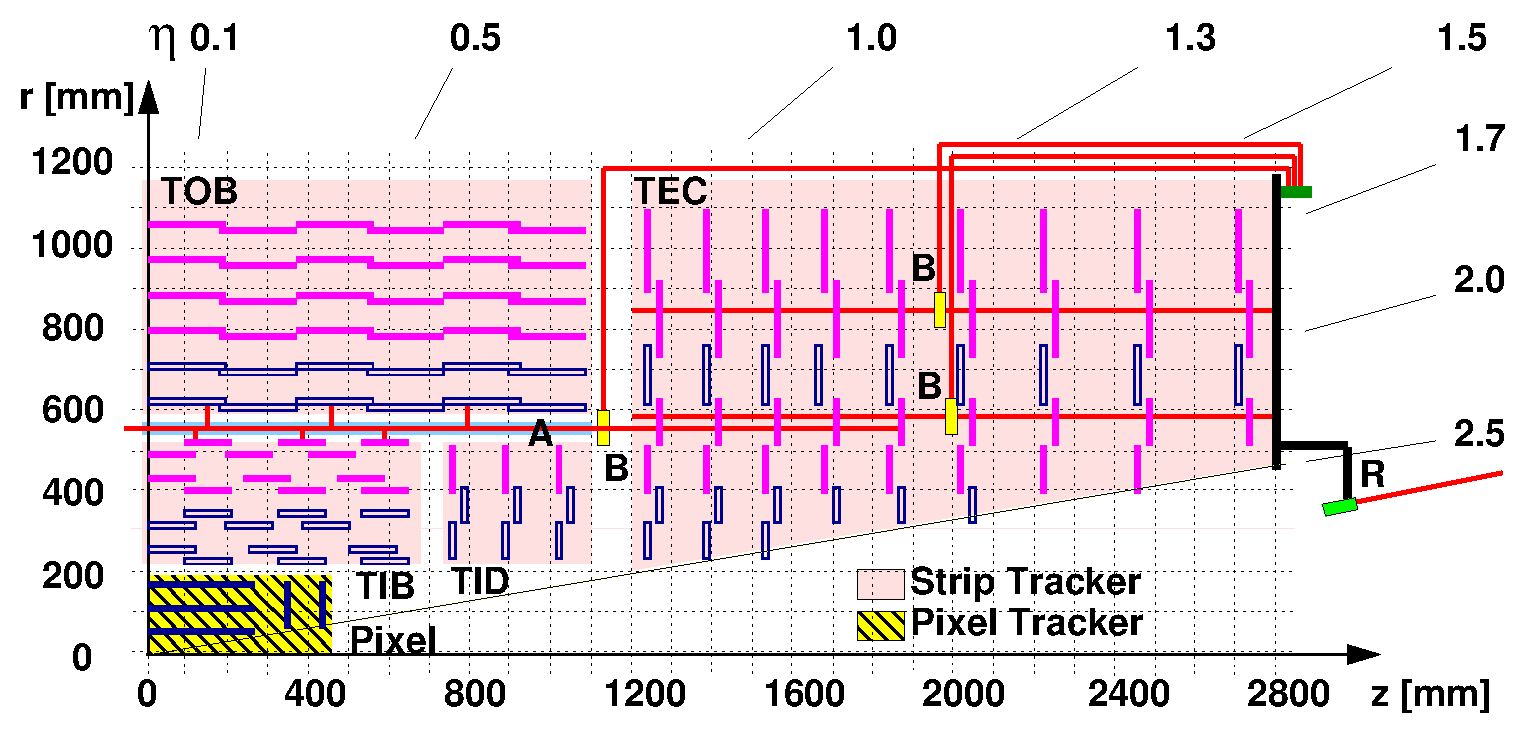
\includegraphics[width=.8\linewidth]{Experiment/figures/TrackerSystemLAS.eps}
\caption[Geometry of the Tracker System]{Tracker cross-section (1/4 of the $z$ view). The pixel tracker is located at the innermost radii of the detector and is labeled in striped yellow. The strip tracker is composed of four regions: Tracker Inner Barrel (TIB), Tracker Outer Barrel (TOB), Tracker End Cap (TEC), and Tracker Inner Disks (TID). The blue pieces are double-sided modules while magenta are single-sided. In addition to the silicon sensors, an infrared laser alignment system is used to provide coarse calibration for the tracker.}
\label{fig:TrackerSystem}
\end{center}
\end{figure}

\begin{figure}[htbp]
\begin{center}
\includegraphics[width=.45\linewidth]{Experiment/figures/MuonTrackEfficiency.pdf}
\includegraphics[width=.45\linewidth]{Experiment/figures/PionTrackEfficiency.pdf}
\caption[Global Track Reconstruction Efficiency at CMS]{Global track reconstruction efficiency of muons (left) and pions (right) for transverse momenta of 1, 10, and 100 $\rm{GeV}/c$. Overall efficiency decreases for smaller $p_T$ and near the edges of the detectable region.}
\label{fig:TrackEfficiency}
\end{center}
\end{figure}

As the tracker subsystem is the only one that can reconstruct vertices, great care is taken to affirm that the numerous pieces of the tracker are aligned to very high precision (ideally smaller than the hit resolution, so $\lesssim10\mu\rm{m}$). After construction, a laser alignment system is used to calibrate the tracker, as well as other subsystems, to account for shifts in orientation. However, this method primarily accounts for large scale misalignments and not individual modules. In sum, there are 9.6 million strips and 66 million silicon pixels spread across over 16000 modules, where the position and orientation of each must be tracked independently both before and during operation of CMS. The only way to get the desired detector position resolution is to use track-based alignment.

After measuring the positions of the various devices during construction and utilizing the laser alignment system, trajectories can be used to further the alignment. Since trajectories should be continuous, small misalignments of the modules will appear as discontinuities in the tracks and measuring their pull. In 2008, when the detector was fully constructed but the beam was not yet running, millions of cosmic muons were tracked through the detector. Computationally, to find the individual corrections, it is equivalent to minimizing a matrix equation for $O(10^5)$ degrees of freedom. Nevertheless, using a combined method of algorithms to find global and local correlations, the positions of the modules were determined to an average precision of 3-4 $\mu$m in the barrel and 3-14 $\mu$m in the endcap in the most sensitive coordinate~\cite{}. Since environmental conditions of operation can cause deviations, similar alignment strategies are used by CMS during data collection.

\subsection{Particle Identification}
\label{sec:ParticleID}

During operation, when the beams collide, all of the subsystems work in tandem to identify different particles by what portions they interact with. Muons and electrons will both record hits in the tracker, but the muon will move through the muon system while electrons stop in the ECAL. Fig.~\ref{fig:CMSSliceWithTracks} shows a diagram with the expected interactions from a sample set of particles. In theory, it seems like this should be simple categorization: only electrons and photons should interact with the ECAL, hadrons will interact with the HCAL, etc. Although it can be this simple, in practice, it is more nuanced. There are roughly 20-30 collisions per crossing and each can have multiple decay products which could deposit energies at similar locations; if a photon strikes the ECAL near an electron, how does CMS disentangle the two? Moreover, the lines between subdetectors aren't quite as strict. For example, neutral pions will commonly decay to two photons and thus could mimic a photon in the ECAL. Alternatively, decay in the ECAL can leak into the HCAL. CMS accounts for these \textit{fake rates} and makes proper identifications by using the \textit{particle-flow algorithm}~\cite{}. 

\begin{figure}[htbp]
\begin{center}
\includegraphics[width=.9\linewidth]{Experiment/figures/CMSSliceWithTracks.png}
\caption[Trajectories and Decays for Particle Identification in CMS]{Transverse slice of CMS with sample trajectories and decays from expected SM particles. Photons (dashed blue) and electrons will deposit their energy in the Electromagnetic Calorimeter, while both neutral (dashed green) and charged hadrons (green) deposit in the Hadronic Calorimeter. Muons (blue) will move through the muon system. All charged particles will interact with the tracker, leaving curved trajectories.}
\label{fig:CMSSliceWithTracks}
\end{center}
\end{figure}

Particle-flow links the output from the different subdetectors to iteratively identify particles. For charged particles, there will be tracks that would align with energy deposits in the calorimeters or the muon system. The hits in the calorimeters are clustered by looking for local maxima and associating nearby elements that are above threshold. In some cases, additional information can be used with the clustering. For example, in the ECAL, electrons will spread energy over a larger area that converted photons. These clusters (or trajectories in the muon system) are then matched to trajectories in the tracker system. Starting with a very tight cut between the two elements, matched particles and their associated hits in the subdetectors are removed from consideration and the algorithm repeats with a looser constraint.

This algorithm removes elements in a particular order\footnote{This is roughly in order of resolution for the expected particle, where each identification has little influence on successive identifications.}, starting with global muons, then electrons and photons, and finishing with jets. Once all particles are reconstructed, the missing transverse energy can be calculated. Finally, isolation can be used to indicate whether a given reconstructed particle is a \textit{prompt}, meaning that it comes from initial interaction. These reconstructed particles form the basic framework of all analyses at CMS. 

\subsection{Triggers}
\label{sec:Triggers}

As specified in Sec.~\ref{sec:LHC}, the intended number of collisions is on the order of 1 billion per second. However, only about 100 events per second can be stored for analysis, so nearly all of the events need to be rejected. Instead of arbitrarily taking data every hundredth of a second, a trigger system is designed so that only potentially interesting events can be captured. To determine what is interesting, data is temporarily stored and filtered by custom electronics. For the first trigger, Level-1, events are only accepted if they either have i) primitive objects from subdetectors that pass $p_T$ or $E_T$ thresholds or ii) global $E_T$ or missing transverse energy ($E_T^{miss}$ or MET). The detector elements with fast time resolution, like the RPCs in the muon system (see Sec.~\ref{sec:MuonSystem}), define these primitive objects. Altogether, the Level-1 trigger procedure, including data transfer and decision making, is designed to be completed within 3.2 $\mu\rm{s}$ and reduces the rate of events to approximately 100 kHz.

After passing the Level-1 trigger, high level triggers (HLTs) apply additional processing are used to further reduce the throughput. Where the Level-1 triggers use primitive objects, HLT cuts on approximately reconstructed objects, applying thresholds for observables like $p_T$, relative isolation in the calorimeters and/or tracker, or $|\eta|$ of the particle. Although a primary purpose of the HLT cuts is to bring the event rate to 100 Hz, these cuts are tuned to be broadly applicable to different analyses, being maximally inclusive to the intended signal while minimizing backgrounds. Each analysis group can then choose from the data that pass the appropriate high level triggers to make a high precision measurement, exclude a theoretical model, or discover a new as-yet undetected particle.

\section{Summary}
\label{sec:expt_summary}

In 2008, after 25 years of construction, the LHC began operation. Within another two years, the combined energy of the beams reached 7 $\rm{TeV}$. In 2011, over 5 $\mathrm{fb}^{-1}$ was collected for 7 $\rm{TeV}$. After increasing the energy to 8 $\rm{TeV}$ in 2012, nearly another 20 $\mathrm{fb}^{-1}$ was collected. This was sufficient to confirm the existence of a Higgs-like boson, appearing to achieve one of the most elusive discoveries in particle physics. This chapter has reviewed the intricacies of the detector itself, explaining the mechanism used to extract relevant information from the decays of trillions of high energy proton collisions. But how exactly was the new particle found in this mountain of data and can we measure its properties? Put bluntly, is this really the Higgs we've been looking for?
\chapter{Higgs Phenomenology at the LHC}
\label{sec:pheno}
\chaptermark{Higgs Phenomenology at the LHC}

\section{Summary}
\label{sec:pheno_summary}
\chapter{Results}
\label{sec:results}
\chaptermark{Results}

\section{Summary}
\label{sec:results_summary}
\chapter{Conclusions and Outlook}
\label{sec:conclusions}
\chaptermark{Conclusions}

Two of the overarching goals behind the construction of the LHC and its detectors were to search for any evidence of the Standard Model Higgs boson and to look for any signs of new physics beyond the Standard Model. Behind the work of hundreds of collaborators and centuries of combined experience, the first goal was achieved. In Sec.~\ref{sec:discovery}, using the $H\rightarrow ZZ\rightarrow 4l$ decay channel over the first run of data for CMS, a Higgs boson near $m_{H}=125.6$ $\rm{GeV}$ was observed to $~7\sigma$ global significance. The matrix element methods outlined in Sec.~\ref{sec:pheno} were crucial to its discovery. The second goal of the LHC, observations that indicate new physics, are a bit more nuanced. At the time of writing, the LHC has yet to observe additional resonances that would be indicative of any theoretical extension of the Standard Model. However, we do have a Higgs boson. If its properties disagree with the expectations of the Standard Model, then particle physicists may have a sign of what the next development will be.

As shown in Sec.~\ref{sec:properties}, the $m_{H}=125.6$ $\rm{GeV}$ Higgs boson appears to match many of the expectations of the Standard Model. In Sec.~\ref{sec:HighMass}, no additional Higgs-like resonances were found in the high mass region. The spin-parity of the Higgs boson should be a spin-0 CP-even particle. Looking at the results of Sec.~\ref{sec:SpinParity}, any spin-1 or spin-2 model is excluded, many at $\geq3\sigma$. From Sec.~\ref{sec:SpinParity} and \ref{sec:OffShellAnom}, the fractional measurements of the anomalous $HVV$ couplings are all in agreement with what should be expected for the Standard Model Higgs boson given current statistical and theoretical limitations. Finally, the total width of the resonance, if anomalously large, would be a strong sign of new physics. But as calculated in Sec.~\ref{sec:WidthResults} and \ref{sec:OffShellAnom} using the combined on-shell and off-shell regions, the width is in agreement with Standard Model expectations. Indeed, when looking at the combination result from all decay channels in CMS, the Higgs boson's signal strength agrees with the predictions, even when split by decay mode as in Fig.~\ref{fig:CombHiggsDecay} or when split by production mode\footnote{There is an excess in $t\bar{t}H$ production, coming largely from $H\rightarrow \gamma\gamma$ and $H\rightarrow WW$.} as in Fig.~\ref{fig:CombHiggsProd}.

\begin{figure}[htbp]
\begin{center}
\includegraphics[width=.45\linewidth]{Conclusions/figures/sqr_mlz_ccc_mH125_decay.pdf}
\includegraphics[width=.45\linewidth]{Conclusions/figures/sqr_m6summary_fitmu.pdf}
\caption[Higgs Boson Signal Strength for CMS Combination Split by Decay Channel]{On left, signal strengths for the combination (vertical black line, with green $\pm1\sigma$ uncertainty bands) and split via subcombinations of bosonic ($H\rightarrow \gamma\gamma$, $H\rightarrow ZZ$, $H\rightarrow WW$) and fermionic ($H\rightarrow \tau\tau$, $H\rightarrow b\bar{b}$) decay modes with horizontal red bars for $\pm1\sigma$ uncertainty around best fit value. On right, deviations of the Higgs boson coupling to fermions and bosons are plotted. Particle masses are taken from \cite{Agashe:2014kda}. Both plots are from \cite{Khachatryan:2014jba}.}
\label{fig:CombHiggsDecay}
\end{center}
\end{figure}

\begin{figure}[htbp]
\begin{center}
\includegraphics[width=.45\linewidth]{Conclusions/figures/sqr_mlz_ccc_mH125_prod.pdf}
\includegraphics[width=.45\linewidth]{Conclusions/figures/sqr_rvrf_scan_2d_all_68.pdf}
\caption[Higgs Boson Signal Strength for CMS Combination Split by Production]{On left, signal strengths for the combination (vertical black line, with green $\pm1\sigma$ uncertainty bands) and split via subcombinations of tags for different production mechanisms (VBF, VH, $t\bar{t}H$, and Untagged) with horizontal red bars for $\pm1\sigma$ uncertainty around best fit value. On right, comparison of signal strength for bosonic ($\mu_{\rm VBF,VH}$) vs fermionic ($\mu_{\rm ggH,ttH}$) couplings split by decay channel, with a cross and $1\sigma$ contour for each decay channel plotted alongside the SM expectations (red and yellow diamond). Both plots are from \cite{Khachatryan:2014jba}.}
\label{fig:CombHiggsProd}
\end{center}
\end{figure}

However, just because results currently agree with the expectations of the Standard Model does not imply that this Higgs boson is The Higgs Boson. The second run of the LHC at $13$ $\rm{TeV}$ is about to begin physics runs, do we have any expectations of what sensitivity we can reach in these property measurements?

For the total Higgs width, the limits are all driven by the modeling of the off-shell region. Improving the theoretical uncertainty in the off-shell region -- particularly in the scale factor for the $gg\rightarrow 4l$ channel -- would necessarily improve the measurement. However, this only goes so far. If the Higgs width is smaller than SM predictions, this could appear in the signal strengths of different decay channels. For large values of the Higgs width, the lack of signal-like events in the off-shell region provides a limit. But because the destructive off-shell interference is proportional to $\sqrt{\Gamma_{H}}$ while signal is proportional to $\Gamma_{H}$, when $\Gamma_{H}\approx\Gamma_{SM}$, this intermediate width region cannot be probed well using the off-shell analysis. No expectations for the total width using $13$ $\rm{TeV}$ simulation has been set, but the measurement is not expected to improved dramatically with more data.

However, the anomalous coupling measurements are statistically limited. In \cite{Anderson:2013afp}, we investigated the sensitivities for anomalous $HVV$ couplings within the lifetime of the LHC (both with and without the anticipated high lumionsity upgrade\footnote{The \textit{HL-LHC} is a high luminosity upgrade for the LHC intended to be built in the coming years. It would increase the lifetime integrated luminosity of the LHC by a factor of 10 \cite{ATLAS:2013hta,CMS:2013xfa,Dawson:2013bba}.}) and a range of considered energies for a future lepton colliders\footnote{Aside from the HL-LHC, there are plans being evaluated for future lepton colliders \cite{Behnke:2013xla,Koratzinos:2013ncw} which would require a choice of beam energy.}. Lepton colliders will have drastically different production preferences than Sec.~\ref{sec:HiggsProduction}, with VBF and VH being the dominant mechanisms. Furthermore, the ratios of production cross sections for an anomalous Higgs boson compared to the SM Higgs boson for VBF and VH will be considerably higher than ggF, so these production mechanisms are important to quantify at the LHC, in addition to $H\rightarrow ZZ$ and $H\rightarrow \gamma\gamma$ decays.

Using {\tt JHUGen} to generate $14$ $\rm{TeV}$\footnote{Run II for the LHC is set to $13$ $\rm{TeV}$, but the design energy of the LHC is $14$ $\rm{TeV}$.} signal MC samples and produce the matrix elements, we followed the discriminant framework outlined in Sec.~\ref{sec:SpinParity}. {\tt POWHEG} and {\tt MadGraph} were used to generate the background events ($q\bar{q}\rightarrow ZZ^{(*)}/Z\gamma^{(*)}/\gamma\gamma^{*}$ + jets for LHC, $e^+e^-\rightarrow ZZ$ for lepton colliders), scaled to account for all backgrounds in the respective production or decay. Then, with physics objects defined similarly as Sec.~\ref{sec:zz4lObjects} and after lepton momenta smearing as used in \cite{Gao:2010qx,Bolognesi:2012mm}, selection requirements were set similar to Sec.~\ref{sec:ZZ4lSelection} for $H\rightarrow ZZ\rightarrow 4l$ or \cite{Khachatryan:2014ira} for $H\rightarrow \gamma\gamma$. The total yields of each decay or production was set for the LHC at $300$ $\rm{fb}^{-1}$ and $3000$ $\rm{fb}^{-1}$ and different beam energies for lepton colliders.

The predicted sensitivities to the CP-odd cross section from these yields is found in Table~\ref{tbl:SnowmassCP} and Fig.~\ref{fig:SnowmassCP}. In summary, sensitivity to CP violation\footnote{In Table~\ref{tbl:SnowmassCP} and Fig.~\ref{fig:SnowmassCP}, the term $f_{CP}$ is used. The translation between $f_{CP}$ and $f_{a3}$ from Sec.~\ref{sec:HVVVertex} is not linear, but they represent the same information.} in the Higgs boson is expected to be on the order of $10^{-4}$ in the HL-LHC or future linear colliders, particularly from VBF and VH production mechanisms. The expected value of $f_{CP}$ for $H\rightarrow ZZ$ decay is very small, around $10^{-5}$ even for large pseudoscalar contributions.

\begin{sidewaystable}[t]
\centering
\footnotesize
\begin{tabular}{|ccc|cc|cc|cc|cc|c|c|c|}
\hline\hline
 &  &  &  \multicolumn{6}{c|}{ $HZZ / HWW$ } &   \multicolumn{2}{c|}{ $Hgg$} &  $HZ\gamma$  &    \multicolumn{2}{c|}{ $H\gamma\gamma$ } \\
\hline
Collider & Energy & ${\mathcal{L}}$ &  \multicolumn{2}{c|}{ $H\to VV^*$ } &  \multicolumn{2}{c|}{ $V^*\to V\!H$}  &  \multicolumn{2}{c|}{ $V^*V^*\to H$} 
                                &  \multicolumn{2}{c|}{  $gg\to H$}  &   $H\to Z\gamma$ & $\gamma\gamma\to H$ &  $H\to\gamma\gamma$  \\
%
       &  $\rm{GeV}$   & fb$^{-1}$ &  $f_{C\!P}$ & $\delta f_{C\!P}$ &  $f_{C\!P}$ & $\delta f_{C\!P}$ &  $f_{C\!P}$ & $\delta f_{C\!P}$ &  $f_{C\!P}$ & $\delta f_{C\!P}$ &   &  &   \\
\hline 
$pp$ & 14\,000   & 300 & 0.18 & 0.06 & $ 6\times\!10^{-4}$ & $4\times\!10^{-4}$ &  $18\times\!10^{-4}$ & $7\times\!10^{-4}$ & -- & 0.50   & ~~ & ~~  & ~~   \\
$pp$ & 14\,000   & 3\,000 & 0.06 & 0.02 & $3.7\times\!10^{-4}$ & $1.2\times\!10^{-4}$ &  $4.1\times\!10^{-4}$ & $1.3\times\!10^{-4}$ & 0.50& 0.16   & \checkmark  & ~~  &  \checkmark \\
$e^+e^-$ & 250   & 250 &  \multicolumn{2}{c|}{ \checkmark}  & $21\times\!10^{-4}$ & $7\times\!10^{-4}$ &   \multicolumn{2}{c|}{ \checkmark}   &  &   & ~~ & ~~  & ~~   \\
$e^+e^-$ & 350   & 350 &  \multicolumn{2}{c|}{ \checkmark}  & $3.4\times\!10^{-4}$ & $1.1\times\!10^{-4}$ &   \multicolumn{2}{c|}{ \checkmark}   &  &   & ~~ & ~~  & ~~   \\
$e^+e^-$ & 500   & 500 &  \multicolumn{2}{c|}{ \checkmark}  & $11\times\!10^{-5}$ & $4\times\!10^{-5}$ &   \multicolumn{2}{c|}{ \checkmark}   &  &   & ~~ & ~~  & ~~   \\
$e^+e^-$ & 1\,000   & 1\,000 &  \multicolumn{2}{c|}{ \checkmark}  & $20\times\!10^{-6}$ & $8\times\!10^{-6}$ &   \multicolumn{2}{c|}{ \checkmark}   &  &   & ~~ & ~~  & ~~   \\
$\gamma\gamma$  & 125 & & \multicolumn{2}{c|}{ \checkmark} &&&&&&&&  \checkmark & \\
\hline\hline
%
\end{tabular}
\caption[Projected Sensitivities for CP-Violating Anomalous Coupling of Higgs Boson at LHC and Future Colliders]{Projected sensitivities for $f_{CP}$ in $HVV$ couplings at $3\sigma$ significance with corresponding uncertainties. Current LHC lifetime projections were found using a beam energy of $14$ $\rm{TeV}$ and integrated luminosity of $300$ $\rm{fb}^{-1}$ or $3000$ $\rm{fb}^{-1}$ including the anticipated high luminosity upgrade. $e^+e^-$ and $\gamma\gamma$ refer to proposed future lepton or photon colliders. Numerical values are calculated for $Hgg$ and $HZZ/HWW$ decays. The $\checkmark$ indicates that a measurement could be done, but its projection was not calculated.}
\label{tbl:SnowmassCP}
\end{sidewaystable}

\begin{figure}[htbp]
\begin{center}
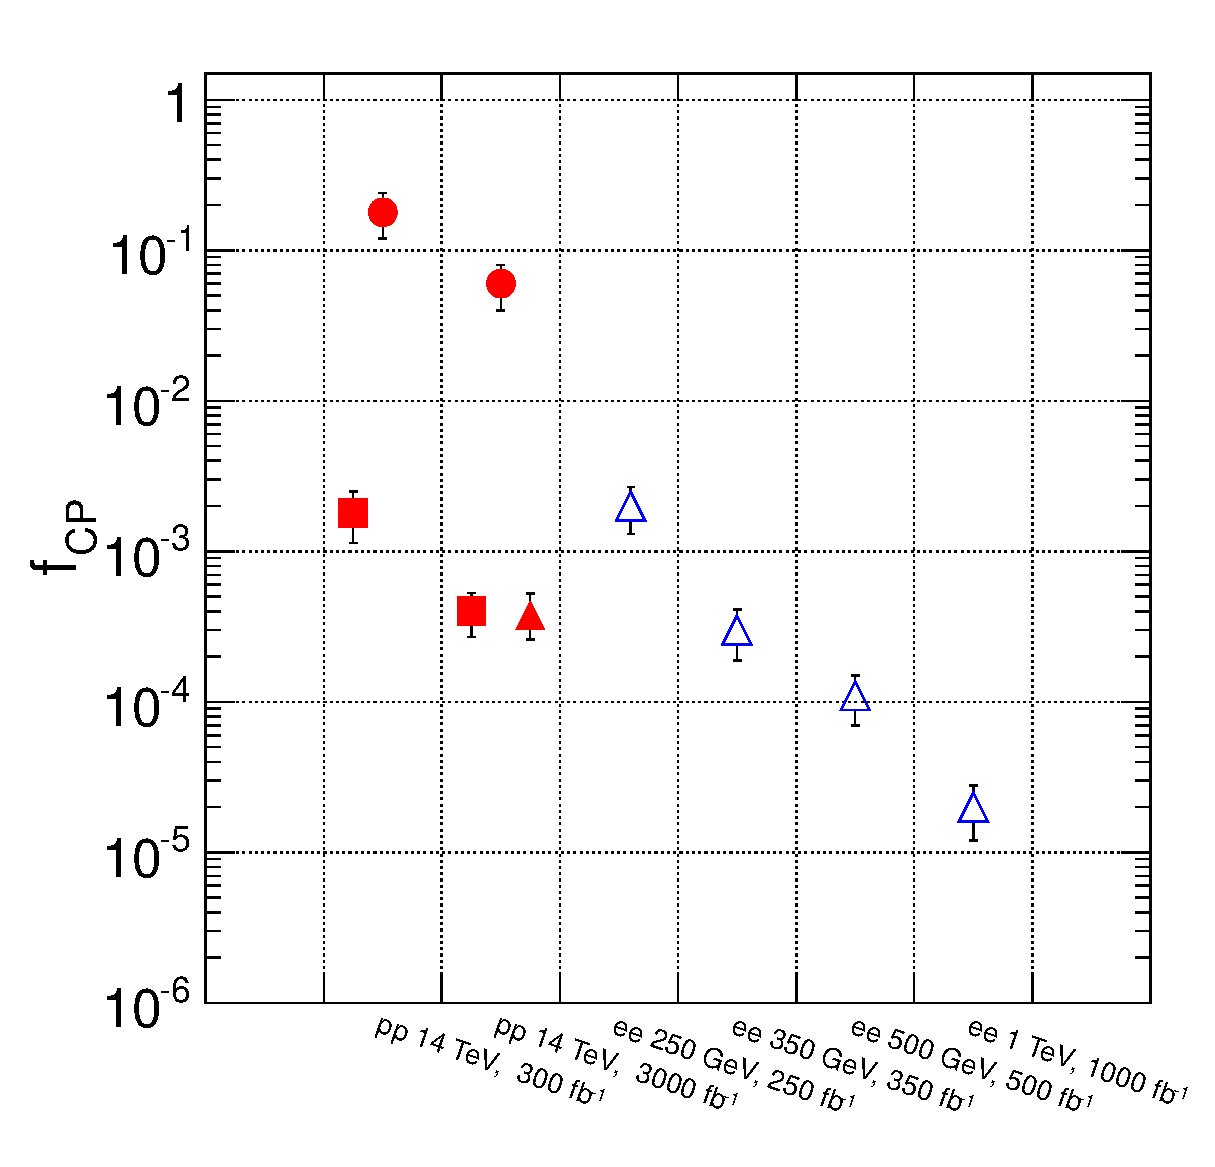
\includegraphics[width=.9\linewidth]{Conclusions/figures/summary_fcp}
\caption[Summary of Precisions for CP-Violating Anomalous Coupling in $HVV$ Vertex at LHC and Future Colliders]{Summary of $f_{CP}$ precisions on the $HVV$ vertex at the LHC (solid red) and proposed future colliders (open blue). VH (triangles) and VBF (square) production methods as well as $H\rightarrow VV$ decays (circles) are shown. Energies and luminosities are listed in the $x$-axis.}
\label{fig:SnowmassCP}
\end{center}
\end{figure}

At the time these sensitivities were projected, the off-shell measurement was not yet designed; these measurements are all from on-shell measurements. If we combine the off-shell anomalous coupling measurement techniques described in Sec.~\ref{sec:OffShellAnom}, the overall measurement of anomalous $HVV$ couplings can become even tighter, especially for VBF production. It is plausible that the sensitivity of $f_{CP}$ could become test some BSM theoretical predictions within the lifetime of the LHC. Until and unless the LHC observes new particles not predicted by the Standard Model, this technique and others like it can provide more concrete information concerning physics beyond the Standard Model.

By any standard, the searches and property measurements of the Higgs Boson should be considered a grand success, both for the Standard Model and the LHC. For their theoretical contribution, Higgs and Englert were jointly awarded the Nobel Prize in Physics in 2013. But the Higgs Boson was the last piece of the Standard Model which -- even with its immense predictive power and precision -- is known to be insufficient to explain all phenomena in particle physics. The next wave of searches, either through direct measurement of new particles or indirectly through precision Higgs boson properties, will aim to answer the current mysteries: What, exactly, is dark matter? What about dark energy? Why is there more matter than antimatter? In short, the question we must answer individually and cosmically: How did we get here and where are we going? That is the solitary goal of all particle physics, even physics in general. Through the LHC and the Higgs boson, we move closer to providing an answer.



%\include{appendix}

%% REFERENCES

% if you use BIBTEX
\bibliographystyle{IEEEtran}
\bibliography{thesis}

\pagebreak
\begin{cv}{{\large Ian Anderson}\\
    {\normalsize Johns Hopkins University, 
      Department of Physics and Astronomy\\
      Email: ianderso@pha.jhu.edu
      \hfill Phone: {\mdseries 717-580-4187} 
    }
}
\fancyhead[RE,LO]{CURRICULUM VITAE}
\newlength{\oldcvlabelwidth}
\newlength{\oldcvlabelsep}

\setlength{\oldcvlabelwidth}{\cvlabelwidth}
\setlength{\oldcvlabelsep}{\cvlabelsep}

\setlength{\cvlabelwidth}{1em}

\begin{cvlist}{Education}
\item \emph{B.S., Physics with Honors}\\
Carnegie Mellon University, September 2005 - June 2009
\item \emph{M.A., Physics}\\
Johns Hopkins University, 2011
\item \emph{Ph.D., Physics}, Expected May 2015\\
  Johns Hopkins University, September 2009 - present  
\end{cvlist}

\setlength{\cvlabelwidth}{0em}
\setlength{\cvlabelsep}{\labelsep}

\begin{small}

\begin{cvlist}{Research Experience}
\item
\begin{itemize}\itemsep=0.25em
	\item Graduate Research, Johns Hopkins University, CMS Collaboration, Fall 2011 - present
         \begin{itemize}
		\item Discovered Higgs boson to very high statistical significance ($\sim7\sigma$) with small number ($\sim 25$) out of billions of potential events
		\item Utilized grid computing and parallel processing over very large datasets ($> 1$ PB)
		\item Developed novel multivariate analyses to measure properties of Higgs production
		\item Produced and validated new Monte Carlo simulator used throughout LHC Experiment
		\item Interpreted data through statistical analysis
		\item Implemented technique to improve measurement of Higgs width by a factor of 200 over prior methods
	\end{itemize}
	\item Monte Carlo Convener for HZZ, CMS Collaboration, 2013 - 2014
	\begin{itemize}
		\item Led and coordinated Monte Carlo Simulation across 20+ research institutions from seven countries
		\item Defined, produced, and validated Monte Carlo Simulations for six different scientific publications
	\end{itemize}
	\item Research Assistant, INFN Bari, CMS Collaboration, Fall 2012
	\begin{itemize}
		\item Interfaced between INFN Bari and other international research institutions
		\item Developed analyses to produce consistency between multiple statistical frameworks
	\end{itemize}
	\item Research Assistant, Johns Hopkins University, USA, Summers 2010 \& 2011
	\begin{itemize}
		\item Implemented software for noise reduction of astronomical observations
	\end{itemize}
	\item Undergraduate Research Assistant, Indiana University, USA, Summer 2008
	\begin{itemize}
		\item Analyzed discrepancies between many-body discrete models and continuous approximations in particle accelerator design
	\end{itemize}
\end{itemize}
\end{cvlist}

\begin{cvlist}{Invited Positions}
\item
\begin{itemize}\itemsep=0.25em
	\item Instructor, CMS Data Analysis School, January 2013
	\begin{itemize}
		\item Created and Organized rigorous week long Data Analysis Exercise for Graduate Students in CMS Collaboration
		\item Taught data analysis techniques common to the $H\rightarrow ZZ$ subgroup of the CMS Experiment
	\end{itemize}
\end{itemize}
\end{cvlist}

\begin{cvlist}{Teaching Experience}
\item
\begin{itemize}\itemsep=0.25em
	\item Head Teaching Assistant, General Mechanics II, Spring 2015
	\item Teaching Assistant, Advanced Physics Lab, Springs 2013 \& 2014
	\begin{itemize}
		\item Designed and validated experimental procedures for upper-level undergraduate physics majors
		\item Taught statistical techniques including model building and error analysis
	\end{itemize}
	\item Teaching Assistant, General Physics II, Springs 2010, 2012, 2013
	\item Teaching Assistant, Special Relativity and Waves, Fall 2011
	\item Teaching Assistant, General Physics I, Falls 2009 \& 2012, Spring 2011
	\item Teaching Assistant, General Physics I Lab, Falls 2009 \& 2012, Springs 2010 \& 2011
\end{itemize}
\end{cvlist}

\begin{cvlist}{Presentations and Talks}
\item
\begin{itemize}\itemsep=0.25em
	\item Pheno 2014. Pittsburgh, PA, May 2014 \\
	``Constraints on the Higgs boson total width using off-shell production in the ZZ decay"
	\item APS April Meeting. Savannah, GA, April 2014 \\
	``Measurement of the properties of a Higgs boson in the four-lepton final state"
	\item CMS WGM 183. Geneva, Switzerland, April 2014 \\
	``Constraints on the Higgs boson width from off-shell $H\rightarrow ZZ$ production"
\end{itemize}
\end{cvlist}

\begin{cvlist}{Publications}
\item
\begin{itemize}\itemsep=0.25em
	\item Selected Refereed Journal Publications
	\begin{itemize}
		\item I.\ Anderson et al., ``Constraining anomalous HVV interactions at proton and lepton colliders", Phys.\ Rev.\ D 89, 035007 
		\item CMS Collaboration, ``Measurement of the properties of a Higgs boson in the four-lepton final state", Phys.\ Rev.\ D 89, 092007
		\item CMS Collaboration, ``Constraints on the Higgs boson width from off-shell production and decay to Z-boson pairs", Phys.\ Lett.\ B 736 (2014) 64 
	\end{itemize}
	\item Submitted Journal Publications
	\begin{itemize}
		\item CMS Collaboration, ``Constraints on the spin-parity and anomalous HVV couplings of the Higgs boson in proton collisions at 7 and 8 TeV", CMS PAS HIG-14-018 (2014)
	\end{itemize}
	\item Papers in Preparation
	\begin{itemize}
		\item CMS Collaboration, ``High mass WW and ZZ Higgs search with full statistics"
		\item	CMS Collaboration, ``Lifetime analysis using Higgs to 4l events"   
	\end{itemize}
\end{itemize}
\end{cvlist}

\begin{cvlist}{Educational Outreach}
\item
\begin{itemize}\itemsep=0.25em
	\item USA Science and Engineering Festival, Aprils 2012 \& 2014
	\begin{itemize}
		\item National biennial science festival with 300k+ attendees
		\item Provided public outreach related to CMS and Experimental Particle Physics
	\end{itemize}
	\item Johns Hopkins Physics Fair, Aprils 2010 - 2015
	\begin{itemize}
    		\item Annual outreach program for local families and children on physics information
	\end{itemize}
	\item Baltimore Area High School Demonstrations, March 2013
	\begin{itemize}
		\item Organized demonstrations for local area high school physics courses
	\end{itemize}
\end{itemize}
\end{cvlist}

\setlength{\cvlabelwidth}{\oldcvlabelwidth}
\setlength{\cvlabelsep}{\oldcvlabelsep}
\end{small}

\end{cv}

\end{document}
